\section{Literature Review}

Fabric classification has been an area of growing interest in the fields of computer vision and material science due to its wide range of applications across industries such as fashion, healthcare, manufacturing, and forensics. With the advancement of deep learning, researchers have been exploring automated methods to accurately identify and classify textile materials using image data.

Traditionally, fabric classification relied on manual techniques and physical testing, but these approaches are time-consuming, prone to human error, and often require specialized equipment. In contrast, image-based classification using deep learning models offers a scalable and efficient alternative that can be used even in real-time applications.

In this section, we review key research contributions that have applied deep learning techniques for fabric classification. The datasets described here, used in these studies are carefully considered, as data quality and diversity are vital to achieving strong model performance. We also provide a detailed discussion of the three papers that were selected and implemented as part of this research work. Each paper highlights a different modeling approach offering valuable insights into the strengths and limitations of current methodologies.

By analyzing these works, we aim to identify the common practices, innovative ideas, and existing challenges in the domain, which in turn have shaped the direction of our proposed methodology.

\subsection{Dataset Overview}

The development of accurate and generalizable deep learning models for fabric classification is heavily dependent on the availability of high-quality, diverse, and well-structured datasets. Each dataset used in this domain captures textile properties from a unique perspective—some focus on fine surface-level textures, others provide microscopic or structural imaging, and some present large-scale image collections labeled through expert-driven taxonomies.

In this section, we present a detailed review of three key datasets that were used in the implementation and evaluation of deep learning models for this research. These datasets have been selected for their relevance, diversity, and their ability to represent different challenges in fabric classification. Each dataset has contributed to our understanding of how fabrics can be categorized based on visual cues, micro-structures, and material properties. The datasets reviewed are described below:

\newpage
\subsubsection{A. Fine-Grained Material Classification Using Micro-geometry and Reflectance~\cite{kampouris2016fine}}

One of the foundational datasets used for fine-grained material classification is based on micro-geometry and reflectance properties. This dataset, introduced by Kampouris et al., captures subtle material differences through high-resolution images that include shape, surface detail, and reflectance captured under varying lighting conditions.

The dataset was developed to aid in distinguishing materials that are visually similar to the human eye but differ in their physical or optical properties. It includes a range of fabrics and other material surfaces, photographed under controlled settings using a multi-light camera rig. Each sample is captured from multiple angles and under multiple lighting directions to collect reflectance fields. This setup allows for capturing texture, gloss, and geometric cues that are often difficult to extract from standard RGB images.

\begin{figure}[H]
    \centering
    \begin{minipage}{0.8\linewidth}
        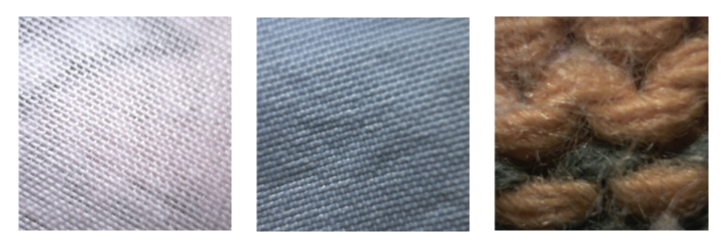
\includegraphics[width=\linewidth]{images/iBugDataset}
    \end{minipage}
    \caption[Sample images from the iBug Fabric Dataset]{Sample images from the iBug Fabric Dataset: (Left) Cotton, (Middle) Polyester, (Right) Wool.}
\end{figure}

What makes this dataset particularly useful for material classification is its emphasis on surface detail and reflectance behavior, rather than color or pattern alone. This makes it ideal for deep learning models that aim to identify materials based on physical characteristics, which are more consistent across environments compared to visual patterns.

Although the dataset covers a broader range of materials beyond textiles, its fabric subset is still highly valuable. It includes fabrics like cotton, wool, denim, and silk—each captured in fine detail—providing strong training data for distinguishing between these visually similar but structurally different materials.

This dataset serves as a strong foundation for deep learning models focused on material classification in fine-grained scenarios and is especially relevant when the goal is to distinguish fabrics based on their structural textures and reflectance rather than color or shape alone.

\subsubsection{B. Optical Coherence Tomography Image Dataset of Textile Fabrics~\cite{sabuncu2022optical}}

The Optical Coherence Tomography (OCT) image dataset of textile fabrics is a unique and specialized dataset that provides high-resolution cross-sectional images of fabric structures. Developed by Sabuncu and Ozdemir, this dataset aims to support material classification tasks through depth imaging and has proven useful for textile engineering, recycling, and forensic analysis.

The dataset includes OCT scans of fabrics made purely from cotton, wool, and polyester. For each material type, three different fabric samples were selected, resulting in a total of nine fabric categories. Using the Thorlabs CAL110C1 OCT system, each sample was scanned at over a hundred random surface locations to generate detailed cross-sectional images, commonly known as B-scans. The scan length was fixed at 2\,mm across all samples, and images were stored in raw \texttt{.png} format without any additional filtering or preprocessing.

\begin{figure}[H]
    \centering
    \begin{minipage}{0.8\linewidth}
        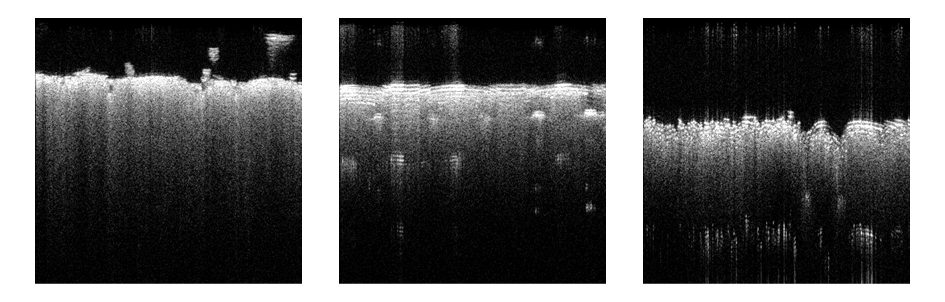
\includegraphics[width=\linewidth]{images/FabricOCTDataset.png}
    \end{minipage}
    \caption[Sample images from the Fabric OCT Dataset]{Sample images from the Fabric OCT Dataset: (Left) Cotton, (Middle) Polyester, (Right) Wool.}
\end{figure}

A key advantage of OCT imaging lies in its ability to reveal internal microstructural features of the fabric that are not visible in standard RGB images. These features include weave patterns, layer thickness, and material density, making OCT particularly valuable for classifying fabrics that may appear visually similar on the surface.

The dataset was structured into three main folders—cotton, wool, and polyester—each containing multiple scans from different fabric pieces of the same material. This setup provides a clean and well-labeled dataset that is suitable for training and testing deep learning models, especially those focused on learning from structural features rather than visual appearance alone.

Overall, the OCT image dataset offers a high degree of consistency and detail, which makes it ideal for tasks that require fine-grained classification of fabric types based on internal structure. Its application extends beyond classification, with potential uses in recycling processes, textile defect detection, and automated quality control in textile production.

\subsubsection{C. TextileNet: A Material Taxonomy-Based Fashion Textile Dataset~\cite{zhong2023textilenet}}

TextileNet is a large-scale, taxonomy-driven dataset designed to support textile material identification using deep learning techniques. Introduced by Shu Zhong et al., it addresses a major gap in existing datasets by providing a structured taxonomy of textile materials, divided into two primary categories: fibres and fabrics. Unlike most fashion-related datasets that often mix fibre and fabric labels or contain vague annotations, TextileNet provides a clearly defined and scientifically grounded label structure developed in collaboration with material science experts.

The dataset is split into two parts: \textit{TextileNet-fibre} and \textit{TextileNet-fabric}, comprising 33 fibre labels and 27 fabric labels, respectively. The total dataset consists of approximately 760,949 images, sourced from Google Images and reconstructed fashion datasets like iMaterialist. The image collection process was carefully curated using keyword-based queries derived from the defined textile taxonomies, ensuring that the dataset reflects real-world clothing items while maintaining a consistent label scheme.

\begin{figure}[H]
    \centering
    \begin{minipage}{0.8\linewidth}
        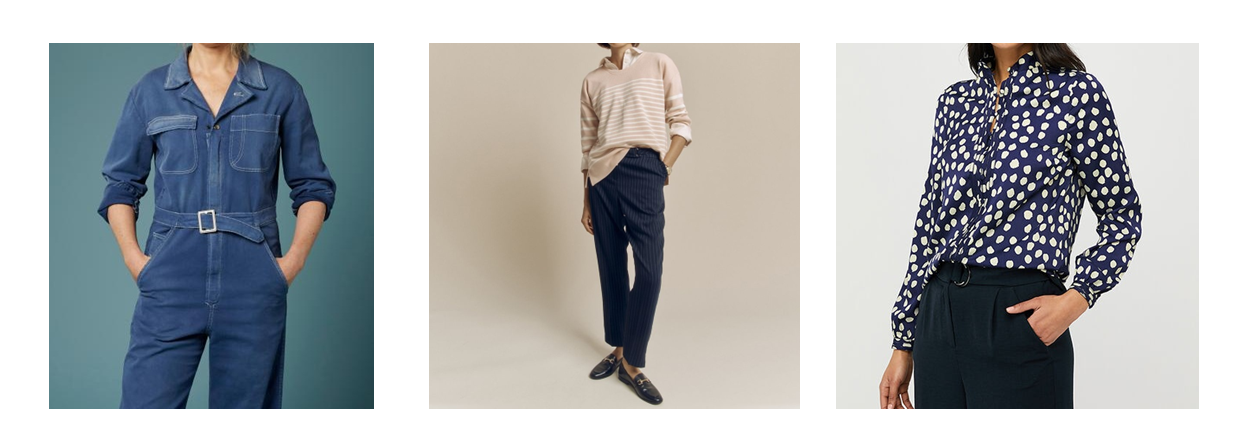
\includegraphics[width=\linewidth]{images/TextileNetDataset.png}
    \end{minipage}
    \caption[Sample images from the TextileNet Dataset]{Sample images from the TextileNet Dataset: (Left) Denim, (Middle) Crepe, (Right) Satin.}
\end{figure}

What makes TextileNet particularly valuable is its taxonomy-based design. The fibre taxonomy includes natural, synthetic, and regenerated fibres such as cotton, wool, polyester, bamboo viscose, and milk casein. The fabric taxonomy, on the other hand, categorizes textiles based on their production method (woven, knitted, non-woven) and includes examples like denim, tweed, velvet, and jersey.

% The dataset has been validated using both Convolutional Neural Networks (CNNs) and Vision Transformers (ViTs), with baseline models achieving over 80\% top-5 accuracy on classification tasks. It not only serves as a resource for textile classification but also supports sustainability-focused goals by enabling traceability of garments back to their fibre and fabric origins—a key step in promoting textile circularity.

Overall, TextileNet is suitable for training robust models that can identify complex fabric compositions in garments, supporting applications in retail, recycling, supply chain management, and sustainable fashion design.